\documentclass{standalone}
\usepackage{tikz}
\usepackage{url}
\usetikzlibrary{shapes.geometric, arrows.meta, positioning, fit}

\begin{document}
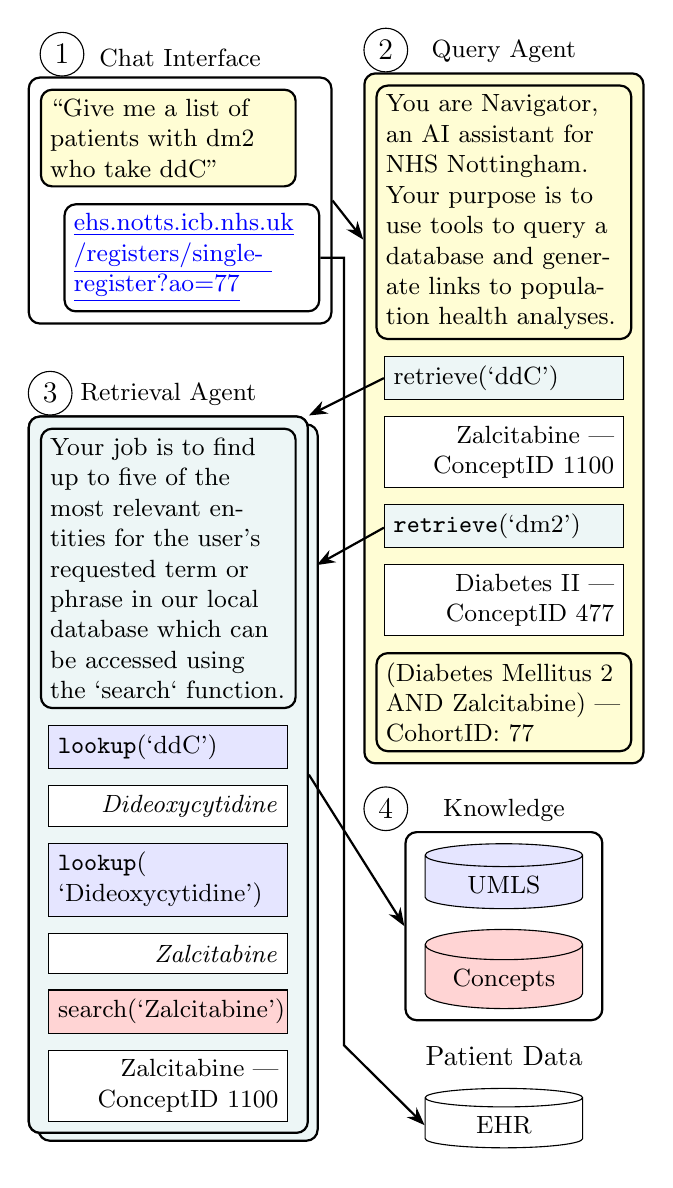
\begin{tikzpicture}[
    node distance=2mm, % vertical spacing between nodes
    innerbox/.style={rectangle, draw, solid, thick, rounded corners, minimum width=1.5cm, minimum height=0.5cm, align=left, text width=3cm, font=\small},
    outerbox/.style={rectangle, draw, thick, rounded corners, minimum width=3.5cm, minimum height=2cm, inner sep=4pt},
    knowledgebox/.style={outerbox, minimum width=2.5cm, minimum height=0.5cm},
    promptbox/.style={innerbox, fill=yellow!17},
    databox/.style={rectangle, draw, solid, minimum width=2.8cm, text width=2.8cm, minimum height=0.5cm, align=left, font=\small, fill=white, align=right},
	retrievetool/.style={rectangle, draw, solid, minimum width=2.8cm, text width=2.8cm, minimum height=0.5cm, align=left, font=\small, fill=teal!7},
	searchtool/.style={rectangle, draw, solid, minimum width=2.8cm, text width=2.8cm, minimum height=0.5cm, align=left, font=\small, fill=red!17},
    umlstool/.style={rectangle, draw, solid, minimum width=2.8cm, text width=2.8cm, minimum height=0.5cm, align=left, font=\small, fill=blue!10},
    linkbox/.style={innerbox, fill=yellow!17},
    arrow/.style={-Stealth, thick},
    data/.style={cylinder, font=\small}
]

% User Interface components
\node[innerbox, fill=yellow!17] (request) {``Give me a list of patients with dm2 who take ddC''};
\node[innerbox, below=of request, xshift=3mm] (response) {
\textcolor{blue}{
\underline{ehs.notts.icb.nhs.uk}
\underline{/registers/single- }
\underline{register?ao=77}}
};

% Processing components
\node[innerbox, right=1cm of request, yshift=-9.43mm]  (prompt) {You are Navigator, an AI assistant for NHS Nottingham. Your purpose is to use tools to query a database and generate links to population health analyses.};
\node[retrievetool, below=of prompt]                (search1)  {retrieve(`ddC')};
\node[databox, below=of search1]                    (result1) {Zalcitabine | ConceptID 1100};
\node[retrievetool, below=of result1]               (search2) {\texttt{retrieve}(`dm2')};
\node[databox, below=of search2]                    (result2) {Diabetes II | ConceptID 477};
\node[innerbox, below=of result2]                   (backend) {(Diabetes Mellitus 2 AND Zalcitabine) | CohortID: 77};


% Retrieval Sub-agent 
\node[innerbox, below=3.05cm of request]  (retrieval0) {Your job is to find up to five of the most relevant entities for the user's requested term or phrase in our local database which can be accessed using the `search` function.};
% \node[databox, below=of retrieval0] (retrieval1) {`ddc'};
\node[umlstool, below=of retrieval0]   (retrieval2) {\texttt{lookup}(`ddC')};
\node[databox, below=of retrieval2]    (retrieval3) {\textit{Dideoxycytidine}};
\node[umlstool, below=of retrieval3]   (retrieval4) {\texttt{lookup}( \\ `Dideoxycytidine')};
\node[databox, below=of retrieval4]    (retrieval5) {\textit{Zalcitabine}};
\node[searchtool, below=of retrieval5] (retrieval6) {search(`Zalcitabine')};
\node[databox, below=of retrieval6]    (retrieval7) {Zalcitabine | ConceptID 1100};

% Grouping boxes
% Grouping boxes with circle labels
\node[outerbox, fit=(request) (response), 
      label={[circle, draw, fill=white, font=\Large, scale=0.75, xshift=-2cm]above:1}, 
      label={[font=\small]above:Chat Interface}] (interface) {};

\node[outerbox, fit=(prompt) (search1) (result1) (search2) (result2) (backend), fill=yellow!17,
      label={[circle, draw, fill=white, font=\Large, scale=0.75, xshift=-2cm]above:2},
      label={[font=\small]above:Query Agent}] (processing) {};

\node[outerbox, fit=(retrieval0) (retrieval2) (retrieval3) (retrieval4) (retrieval5) (retrieval6) (retrieval7), fill=teal!7,
      label={[circle, draw, fill=white, font=\Large, scale=0.75, xshift=-2cm]above:3},
      label={[font=\small]above:Retrieval Agent}] (retrieval) {};

% NEW STAGGERED RETRIEVAL BOX
\node[outerbox, xshift=1.25mm, yshift=-1mm, fit=(retrieval0) (retrieval2) (retrieval3) (retrieval4) (retrieval5) (retrieval6) (retrieval7), fill=teal!7] (retrieval_stagger) {};
\coordinate (retrieval_stagger_top_right) at ([xshift=5mm,yshift=5mm]retrieval.north east);
\coordinate (retrieval_stagger_bottom_left) at ([xshift=5mm,yshift=-5mm]retrieval.south west);

% Re-draw so its in front of the other box lol...
\node[outerbox, fit=(retrieval0) (retrieval2) (retrieval3) (retrieval4) (retrieval5) (retrieval6) (retrieval7), fill=teal!7] (retrieval) {};


%%% DUPLICATES FOR PLOTTING OVER THE BACKGROUND BOXES -- KEEP IN SYNC %%%
\node[innerbox, below=3.05cm of request]  (aretrieval0) {Your job is to find up to five of the most relevant entities for the user's requested term or phrase in our local database which can be accessed using the `search` function.};
% \node[databox, below=of retrieval0] (aretrieval1) {`ddc'};
\node[umlstool, below=of retrieval0]   (aretrieval2) {\texttt{lookup}(`ddC')};
\node[databox, below=of retrieval2]    (aretrieval3) {\textit{Dideoxycytidine}};
\node[umlstool, below=of retrieval3]   (aretrieval4) {\texttt{lookup}( \\ `Dideoxycytidine')};
\node[databox, below=of retrieval4]    (aretrieval5) {\textit{Zalcitabine}};
\node[searchtool, below=of retrieval5] (aretrieval6) {search(`Zalcitabine')};
\node[databox, below=of retrieval6]    (aretrieval7) {Zalcitabine | ConceptID 1100};

\node[innerbox, right=1cm of request, yshift=-9.43mm]  (aprompt) {You are Navigator, an AI assistant for NHS Nottingham. Your purpose is to use tools to query a database and generate links to population health analyses.};
\node[retrievetool, below=of prompt]                (asearch1)  {retrieve(`ddC')};
\node[databox, below=of search1]                    (aresult1) {Zalcitabine | ConceptID 1100};
\node[retrievetool, below=of result1]               (asearch2) {\texttt{retrieve}(`dm2')};
\node[databox, below=of search2]                    (aresult2) {Diabetes II | ConceptID 477};
\node[innerbox, below=of result2]                   (abackend) {(Diabetes Mellitus 2 AND Zalcitabine) | CohortID: 77};


%%%%%%%%%%%%%%%%%%%%%%%%%%%%%%%%%%%%%%%%%%%%%%%%%%%%%%%%%%%%%%%%%%%%%%%%%%


% Define both database nodes
\node[data, aspect=0.25, draw, shape border rotate=90, minimum height=1, minimum width=2cm, below=1cm of processing,  fill=blue!10] (umls) {UMLS};
\node[data, aspect=0.25, draw, shape border rotate=90, minimum height=1, minimum width=2cm, below=0.25cm of umls, fill=red!17] (concept) {Concepts};

% Patient Data
\node[data, aspect=0.25, draw, shape border rotate=90, minimum height=1, minimum width=2cm, below=1cm of concept] (ehr) {EHR};

% Then the data layer grouping box that fits both
% \node[knowledgebox, fit=(umls) (concept), label=above:Knowledge] (data) {};
\node[knowledgebox, fit=(umls) (concept),
      label={[circle, draw, fill=white, font=\Large, scale=0.75, xshift=-2cm]above:4},
      label={[font=\small]above:Knowledge}] (data) {};

% TODO make invis box
\node[knowledgebox, draw=none, fit=(ehr), label=above:Patient Data] (patientdata) {};
\node[knowledgebox, draw=none, fit=(ehr)] (patientdata) {};



% Arrows
% \draw[arrow] (ehr.north) |- ++(-3.125, 1) |- (response.east);
% \draw[arrow] (retrieval2.east) -- (umls.west);
% \draw[arrow] (retrieval3.east) -- (umls.west);
% \draw[arrow] (retrieval4.east) |- ++(3, 0) -- (ehr.south);
% \draw[arrow] (backend.south) -- (ehr.north);

\draw[arrow] (interface.east) -- (processing);

% \draw[arrow] (processing.west) -- (retrieval.north east);
\draw[arrow] (search1.west) -- (retrieval.north east);
\draw[arrow] ([yshift=-19mm]search1.west) -- ([yshift=-19mm, xshift=1mm]retrieval.north east);


% \draw[arrow] (search2.west) -- (retrieval_stagger.north east);

% sub-agent dashed-lines
\draw[arrow] (retrieval.east) -- (data.west);

\draw[arrow] (response.east) --  ++(3mm,0) -- ++(0,-10cm) -- (ehr.west);

\end{tikzpicture}
\end{document}

